\marginpar{VL am 29.04.19} 
\section*{Vorbemerkungen}
\begin{itemize}
	\item Ilias: MaxPlus2019
	\item Vorlesungsart: Tafel + Beiblätter
	\item Prüfung: mündlich, Termine über das ganze Jahr möglich
\end{itemize}

\section{Einleitung}
Grundaufgaben zur Steuerungs- und Regelungstechnik:
\begin{itemize}
	\item Prozessmodellierung
	\item Analyse (Simulation)
	\item Synthese von Regelungen und Steuerungen 
\end{itemize}
Grundlage: \underline{Systemtheorie}

\subsection{Systemklassifikation}
\begin{itemize}
	\item Systemeinteilung nach den wesentlichen Prozessvorgängen möglich (\beiblatt{1-1})
	\item Zuordnung Vorgänge - Prozesstypen (\beiblatt{1-2})
	\item Voraussetzung für sinnvolle Prozessbeschreibung
\end{itemize}

\includepdf[pages={5,6}]{material/AEH_2019.pdf}

\subsubsection{Festlegung des Abstraktionsniveaus}
\properparagraph{Beispiele}
\begin{enumerate}
	\item \textbf{Aufzug}
		\begin{figure}[H]
			\centering
			\includegraphics[width=0.1\textwidth]{img/2019_04_29/abb1.tikz}
		\end{figure}
		
		\underline{Kontinuierliche Vorgänge}
		
		(z.B. Anfahren, Fahren, \ldots)
		$\Rightarrow$ kontinuierliche Modelle (z.B. DGL)
		
		$\Downarrow$ Abstraktion (z.B. Bedienersicht)
		
		\underline{Sequentielle Vorgänge}
		
		(z.B. diskrete Positionsvariablen)
		
		$\Rightarrow$ diskrete Modelle (z.B. Automat)
	\item \textbf{Tank}
	
		\beiblatt{1-3}
		\begin{figure}[H]
			\centering
			\includegraphics[page=7,scale=0.5]{material/AEH_2019.pdf}
		\end{figure}
		
		Abstraktion bedingt durch die AT-Aufgabe und/oder die Randbedingungen (z.B. Aktorik/Sensorik).
		
		Also: Modellierung kombiniert Aufgaben(Ziele) und Prozesswissen(Physik, Randbedingungen)
\end{enumerate}


\subsubsection{Wissensmodellierung und Verarbeitung}
\beiblatt{1-4}
\begin{figure}[H]
	\centering
	\includegraphics[page=8,scale=0.5]{material/AEH_2019.pdf}
\end{figure}

\subsection{Begriffsbestimmungen}
Erforderlich zur Modellformalisierung

Zentrale Begriffe:
\begin{itemize}
	\item System 
	\item Zustand
	\item Ereignis 
	\smash{\raisebox{.5\dimexpr2\baselineskip+4\itemsep+2\parskip}{$\left.\rule{0pt}{.5\dimexpr3\baselineskip+3\itemsep+3\parskip}\right\}\text{Dynamisches System}$}}
\end{itemize}

\beiblatt{1-5}
\includepdf[pages={9}]{material/AEH_2019.pdf}

\properparagraph{Beispiel Tank (Dynamisches System)}

\begin{figure}[H]
	\centering
	\includegraphics[width=0.6\textwidth]{img/2019_04_29/abb2.tikz}
\end{figure}

\begin{figure}[H]
	\centering
	\includegraphics[width=0.6\textwidth]{img/2019_04_29/abb3.tikz}
\end{figure}

\underline{Ereignisse}
\begin{itemize}
	\item \textbf{autonom}: (Größenänderung aufgrund interner Zustandsübergänge)
	\item \textbf{gesteuert}: (Größenänderung aufgrund externer Stellsignale)
\end{itemize}

\properparagraph{Beispiel Zulaufventil}

\begin{figure}[H]
	\centering
	\includegraphics[width=0.6\textwidth]{img/2019_04_29/abb4.tikz}
\end{figure}

\underline{In dieser Vorlesung}

Zwei besondere Ausprägungen dynamischer Systeme betrachtet:
\begin{enumerate}
	\item Ereignisdiskrete Systeme
	\smash{\raisebox{-.5\dimexpr1\baselineskip+4\itemsep+2\parskip}{$\left.\rule{0pt}{.5\dimexpr2\baselineskip+3\itemsep+3\parskip}\right\}\text{Dynamisches System}$}} 
	\item Hybride Systeme 
\end{enumerate}

\underline{Dynamisches System}

\begin{figure}[H]
	\centering
	\resizebox{!}{!}{\includegraphics[width=\textwidth]{img/2019_04_29/abb5.tikz}}
\end{figure}

\properparagraph{Inhalte der Vorlesung}

\begin{itemize}
	\item Ereignisdiskrete Systeme: 
	\begin{itemize}
		\item Modelltypen und Prozessmodellierung
		\item Analyse und Simulation
		\item Spezifikation und Synthese von Steuerungen
	\end{itemize}
	\item Hybride Systeme
	\begin{itemize}
		\item Modellierung
		\item Simulation, Analyse, Steuerung
	\end{itemize} 
\end{itemize}

\subsection{Beispiel: gesteuerter Chargenprozess}
Prozessgeführte Ablaufsteuerung (Struktur siehe \beiblatt{1-6})

\begin{figure}[H]
	\centering
	\includegraphics[page=10,scale=0.5]{material/AEH_2019.pdf}
\end{figure}


\underline{Prinzip}

Einfüllen \textrightarrow Heizen \textrightarrow Entleeren einer Produktmenge(= Charge) [Füllhöhe $h$, Temperatur $\vartheta$] mittels der Stellgrößen [Ein- und Auslassventile $v_1$, $v_2$, Heizung $H$] durch eine diskrete Steuerung.